\documentclass[UTF8]{gyh}

\usepackage{amsmath}
\usepackage{cases}
\usepackage{cite}
\usepackage[margin=1in]{geometry}
\geometry{a4paper}
\usepackage{fancyhdr}
\usepackage{listings} % 添加 listings 宏包以使用 lstlisting 环境
\pagestyle{fancy}
\usepackage{graphicx}
\usepackage{float}
\usepackage[hidelinks]{hyperref}


\title{系统开发工具基础实验报告一}
\author{古宇恒}
\date{\today}
\pagenumbering{arabic}

\begin{document}

\fancyhead[C]{版本控制\ Git}
\fancyfoot[C]{\thepage}

\maketitle
\tableofcontents
\newpage

\section{摘要}
本实验报告将实践版本控制 Git 的使用, Git 的用处,其实就是合并很多人写的代码,并对代码加以版本进行控制,记录代码的编写过程与编写思路。因此,学会使用 Git 是十分有必要的。

\section{Git 基础命令}

虽然现代的 IDE 都自带图形化的 Git 管理界面,比如微软的 VSCode 、Jetbrains 的 WebStorm、CLion、IDEA 等 IDE,都有方便的 Git 管理功能,甚至自带 AI 自动提交功能。同时,GitHub Desktop 也是一款图形化的 Git 应用,也不需要输入任何指令来使用 Git。即便如此,学习基本的 Git 指令依然是必须的,故这里只讲解 Git 指令使用

\subsection{查看 Git 帮助信息}
输入以下指令,可以查看 Git 某个指令的使用方法,或者展示 Git 的所有存在的指令。
\begin{lstlisting}
git help <命令>
\end{lstlisting}
例如,你想要查看 “git branch” 指令的用法,只需要输入 “git help branch” 指令,就可以查询此指令的用法。如图,在输入帮助指令后,帮助文档将使用 vim 直接为你打开,使用方向键或 PgUp、PgDn 翻页,观看完毕后输入 :wq 即可退出。
\begin{figure}[H]
\centering
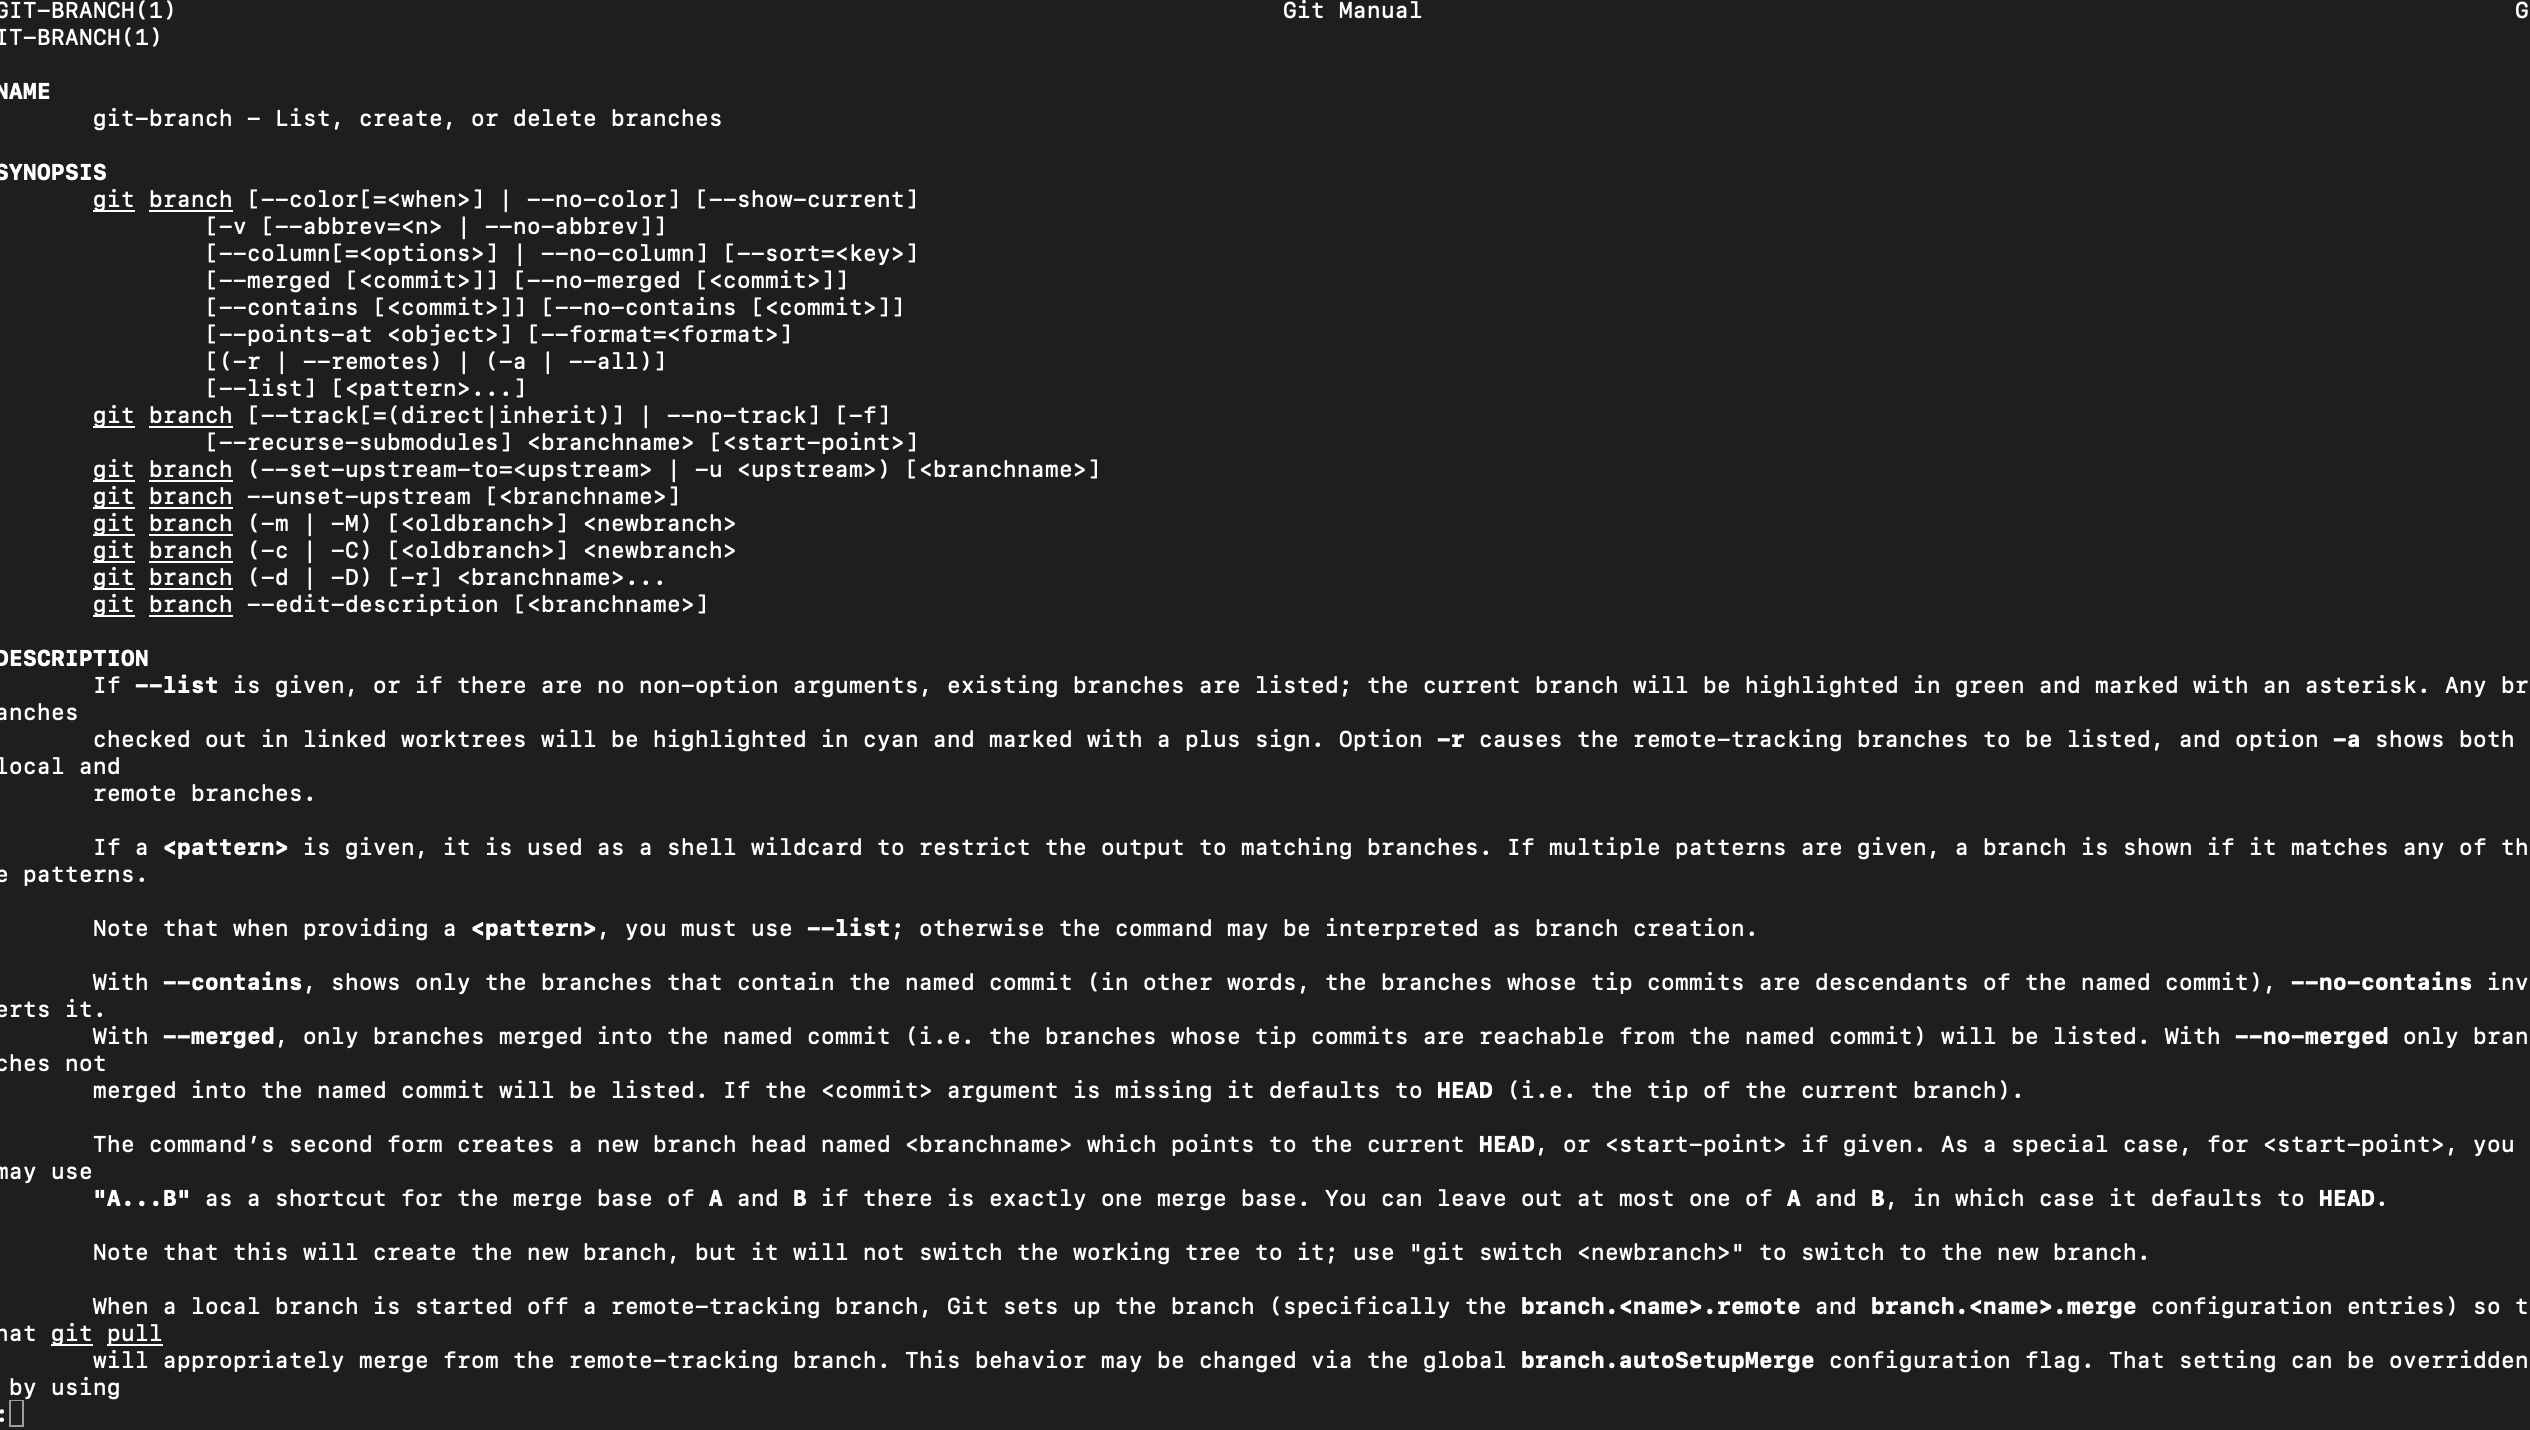
\includegraphics[scale=0.18]{img/img1.png}
\caption{Git 帮助界面}
\end{figure}

\section{Git 仓库操作相关命令}

\subsection{Git 仓库初始化}
该命令用于在当前目录初始化一个新的 Git 仓库。执行后会创建一个 “.git” 子目录,其中包含所有必需的仓库文件。一般这个文件是隐藏文件,无法直接看到。
\begin{lstlisting}
git init
\end{lstlisting}

\subsection{Git 克隆仓库}
这个命令用于从一个已存在的远程仓库克隆一个副本到本地,并且建立一个本地仓库。
\begin{lstlisting}
git clone <仓库地址>
\end{lstlisting}

\subsection{Git 添加提交文件}
该命令将工作区的文件修改添加到暂存区(index),为下一次提交(commit)做准备。
\begin{lstlisting}
# 添加指定文件
git add <文件名>

# 添加所有修改过的文件
git add .
\end{lstlisting}

\subsection{Git 提交}
该命令将暂存区的内容提交到本地仓库,并生成一个新的版本快照。
\begin{lstlisting}
git commit -m "你的描述"
\end{lstlisting}
而有关你的提交描述,最好遵循一个规范,尤其是在团队开发的时候,优秀的提交描述能够很好的让你的合作者理解你所做的事情和你写的代码。一般而言,我们的提交格式是这样的:
\begin{lstlisting}
[<类型>](<涉及模块>) <正文>
\end{lstlisting}
其中,类型是指你的提交所做的事情的分类,比如这是对代码 bug 的修复(fix)还是新增了功能(feat)亦或是代码重构(refactor)。涉及模块则是你所修改的代码所属的模块,正文则需要你来简述你具体在提交中做了什么。虽然看起来这句话没什么用,但是如果你的提交中代码修改量非常大,这一句话对其他人理解你的想法是非常有作用的,因此一定要重视提交描述。

\subsection{Git 获取仓库状况}
该命令用于查看工作区和暂存区的状态,显示哪些文件被修改、暂存或未被跟踪。具体看起来是什么样的,可以看下面的图。
\begin{lstlisting}
git status
\end{lstlisting}
\begin{figure}[H]
\centering
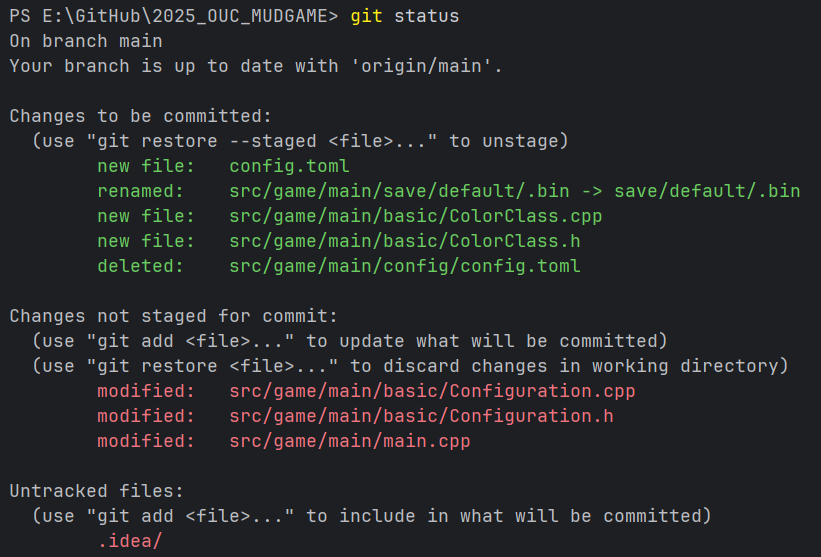
\includegraphics[scale=0.5]{img/img2.png}
\caption{仓库状况展示界面}
\end{figure}


\subsection{Git 查看日志}
该命令用于显示从最近到最远的提交历史记录。它会显示每个提交的信息,包括但不限于提交者、邮箱、提交id、提交描述等信息。如果太长就会切换成 vim 来显示这些信息,使用方法和之前的查看帮助信息是一样的。
\begin{lstlisting}
git log
\end{lstlisting}

\subsection{Git 查看文件差异}
该命令用于显示工作区与暂存区、或两个提交之间的内容差异。
\begin{lstlisting}
# 查看工作区与暂存区的差异
git diff

# 查看暂存区(也就是本地仓库的修改)与最新提交的差异
git diff --staged
\end{lstlisting}

\section{分支相关操作}

在编程过程中,你的软件可能因为要适应其他的运行环境,某些代码需要改版,甚至重写,但是它本质上依然是同一个项目,这时候你就可以使用分支操作来新建一个这个仓库的分支了。事实上,每一个仓库都有分支,只不过分支在你手动创建新的之前只有一个,那就是主分支。比如,GitHub 的默认主分支叫 main ,有些 IDE 的 git 则是 master ,需要仔细观察。

\subsection{Git 分支命令}
这些命令用于列出、创建或删除分支。
\begin{lstlisting}
# 列出所有本地分支
git branch

# 创建一个新分支
git branch <分支名>

# 删除一个分支
git branch -d <分支名>
\end{lstlisting}

\subsection{Git 签出分支}
这个命令用于切换到不同的分支。在较新的Git版本中,推荐使用`git switch`。
\begin{lstlisting}
# 切换到已存在的分支
git checkout <分支名>

# 创建并切换到新分支
git checkout -b <分支名>
\end{lstlisting}

\subsection{Git 合并分支}
这个命令用于将指定分支的历史合并到当前分支。
\begin{lstlisting}
git merge <需要合并的分支名>
\end{lstlisting}

\section{远程仓库相关操作}

\subsection{Git 远程仓库操作}
这个命令用于管理与远程仓库的连接。
\begin{lstlisting}
# 列出所有远程仓库的简称
git remote -v

# 添加一个新的远程仓库
git remote add <仓库简称> <url>
\end{lstlisting}

\subsection{Git 仓库拉取}
这个命令从远程仓库下载最新的提交历史和对象,但不会自动合并到你当前的工作中。
\begin{lstlisting}
git fetch <远程名称>
\end{lstlisting}

\subsection{Git 请求更新}
这个命令相当于 git fetch 和 git merge 的组合,它从远程仓库获取最新版本并自动合并到本地当前分支。
\begin{lstlisting}
git pull <远程名称> <分支名>
\end{lstlisting}

\subsection{Git 推送}
该命令将本地分支的提交推送到远程仓库。
\begin{lstlisting}
git push <远程名称> <分支名>
\end{lstlisting}

\section{撤销提交、回滚相关操作}

\subsection{Git 回退提交}
该命令用于重置当前HEAD到指定状态,可以用来撤销提交。它会移动HEAD指针,并可能修改暂存区和工作区。其实这就是 Git 中的后悔药,挽回你给仓库提交的错误代码。
\begin{lstlisting}
# 回退到上一个版本,保留工作区修改
git reset --soft HEAD^

# 回退到上一个版本,并丢弃所有修改
git reset --hard HEAD^
\end{lstlisting}

\subsection{Git 撤销提交}
该命令通过创建一个新的提交来撤销指定的提交,这是一种更安全的回滚方式,因为它不会改变项目历史。表现为前面几个 commit 消失了,但是修改都跑到 revert 提交里了。
\begin{lstlisting}
git revert <提交id>
\end{lstlisting}

\subsection{Git 保存本地修改}
该命令用于临时保存当前工作区和暂存区的修改,让工作目录变干净。
\begin{lstlisting}
# 将修改暂存起来
git stash

# 恢复最近一次暂存的修改并从暂存列表中移除
git stash pop
\end{lstlisting}

\section{Git 使用指令修改配置}

\subsection{Git 设置用户名和邮箱}
在提交代码时,需要署名,因此需要设置用户名和邮箱,方便后面分辨提交信息。
\begin{lstlisting}
# 设置用户名
git config --global user.name 你的名字

# 如果有的话,设置密码
git config --global user.password 密码

# 设置邮箱
git config --global user.email "邮箱"
\end{lstlisting}

\subsection{Git 设置 http/https 代理}
在一些情况下,想要访问远程仓库,需要通过代理,可以通过如下方式设置代理。
\begin{lstlisting}
# http 代理
git config --global http.proxy http://127.0.0.1:1080

# https 代理
git config --global https.proxy https://127.0.0.1:1080
\end{lstlisting}

\end{document}